
Neste seção, descrevemos o possível impacto econômico da Pandemia de COVID-19, contextualizada na Seção~\ref{introducao:pandemia}, verificando mensalmente se o volume transacionado foi próximo ou não no volume esperado.

\section{Cenário geral}

Nessa seção, descrevemos os dados da base totalizados mensalmente de forma agregada.

\begin{figure}[htb]
	\centering
    \caption{Valor total transacionado por mês no período analisado}
    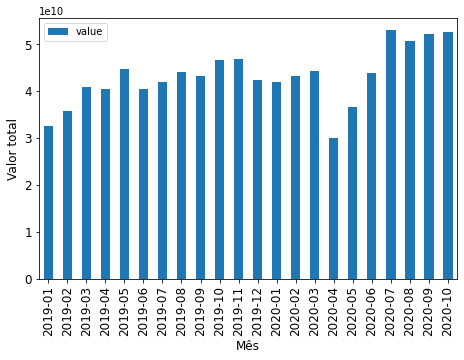
\includegraphics[scale=0.7]{images/base-de-dados-18.1-valor-mensal-total.png}
    \label{fig:pandemia:base-de-dados-18.1-valor-mensal-total}
    \fdadospesquisa
\end{figure}

\begin{figure}[htb]
	\centering
    \caption{Comparação do valor total transacionado por mês entre 2019 e 2020 (Parte 4)}
    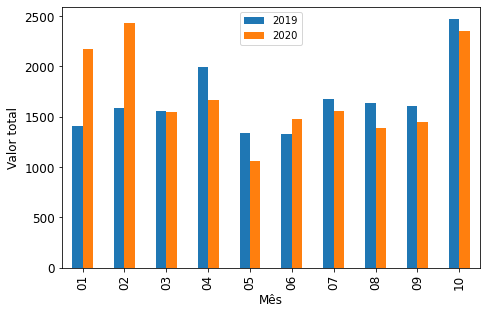
\includegraphics[scale=0.7]{images/base-de-dados-19.1-comparacao-valor-mensal-total.png}
    \label{fig:pandemia:base-de-dados-19.1-comparacao-valor-mensal-total}
    \fdadospesquisa
\end{figure}

A Figura~\ref{fig:pandemia:base-de-dados-18.1-valor-mensal-total} mostra o valor total transacionado em cada mês entre janeiro de 2019 e outubro de 2020, onde é visível um menor valor transacionado principalmente em abril e maio de 2020.

\begin{table}[htb]
\centering
\caption{Variação entre o valor transacionado para cada mês em 2020 em relação a 2019}
\label{tab:comparacao-valor-mensal-total}
\begin{tabular}{lr}
\toprule
Mês & Variação \\
\midrule
Janeiro &   25.49\% \\
Fevereiro & 14.58\% \\
Março &     12.71\% \\
Abril &    -12.24\% \\
Maio &     -11.24\% \\
Junho &      9.20\% \\
Julho &     11.64\% \\
Agosto &     7.52\% \\
Setembro &  17.02\% \\
Outubro &    3.33\% \\
\bottomrule
\end{tabular}
\fdadospesquisa
\end{table}

A Figura~\ref{fig:pandemia:base-de-dados-19.1-comparacao-valor-mensal-total} mostra uma comparação dos valores mensais transacionados em 2020 em relação aos valores mensais de 2019. Verifica-se então que os meses de abril e maio tiveram um valor total transacionado menor no ano de 2020, cuja variação está descritos em detalhes na Tabela~\ref{tab:comparacao-valor-mensal-total}.

Como descrito na Seção~\ref{introducao:pandemia}, os meses de março e abril marcam exatamente o início do isolamento e das quarentenas no Brasil, e a aparentemente o impacto econômico nesses momentos foi mais importante.

Aplicando uma regressão linear a partir dos dados entre janeiro de 2019 e fevereiro de 2020 é possível obter uma da previsão de valor transacionado para os meses seguintes e então comparar com o valor obtido nos meses seguintes: A Figura~\ref{fig:pandemia:base-de-dados-18.2-valor-total-vs-previsao} mostra os valores obtidos em relação aos valores previstos, detalhados na Tabela~\ref{tab:pandemia:valor-total-vs-previsao}.

A partir desses dados, é possível verificar que no período entre março e junho de 2020 o valor transacionado total foi menor que o previsto, verificando uma retomada posterior.

\begin{figure}[htb]
	\centering
    \caption{Valor total transacionado por mês comparado com a previsão para o período analisado}
    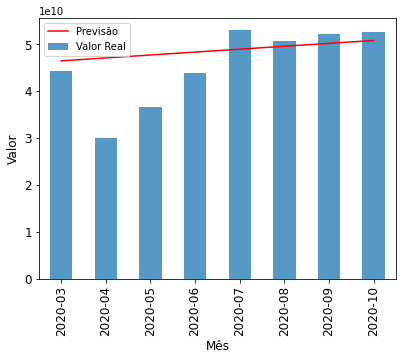
\includegraphics[scale=0.7]{images/base-de-dados-18.2-valor-total-vs-previsao.png}
    \label{fig:pandemia:base-de-dados-18.2-valor-total-vs-previsao}
    \fdadospesquisa
\end{figure}

\begin{table}[htb]
\centering
\caption{Variação entre o valor transacionado para cada mês em relação ao previsto após o início da pandemia}
\label{tab:pandemia:valor-total-vs-previsao}
\begin{tabular}{lr}
\toprule
Mês & Variação \\
\midrule
Março &     -4.46\% \\
Abril &    -36.22\% \\
Maio &     -23.11\% \\
Junho &     -9.15\% \\
Julho &      8.28\% \\
Agosto &     2.09\% \\
Setembro &   4.18\% \\
Outubro &    3.46\% \\ \hline
\textbf{Total} & -6.58\% \\
\bottomrule
\end{tabular}
\fdadospesquisa
\end{table}

\section{Cenário regional}

\begin{figure}[htb]
	\centering
    \caption{Valor total transacionado por região no período analisado}
    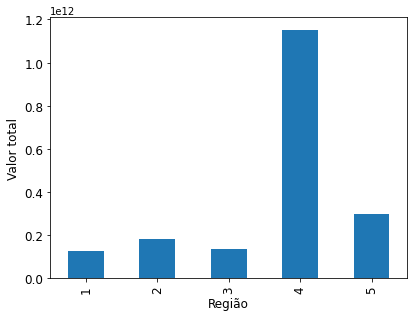
\includegraphics[scale=0.7]{images/base-de-dados-11.1-valor-total-por-regiao.png}
    \label{fig:pandemia:base-de-dados-11.1-valor-total-por-regiao}
    \fdadospesquisa
\end{figure}

\begin{figure}[htb]
	\centering
    \caption{Valor trimestral transacionado por região no período analisado}
    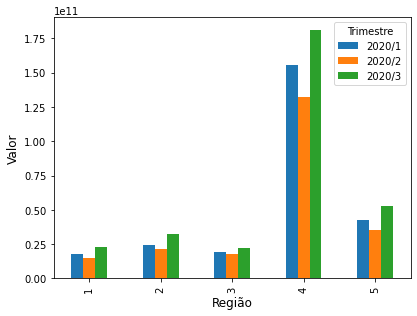
\includegraphics[scale=0.7]{images/base-de-dados-21.1-valor-trimestral-por-regiao.png}
    \label{fig:pandemia:base-de-dados-21.1-valor-trimestral-por-regiao}
    \fdadospesquisa
\end{figure}

\begin{table}[htb]
\centering
\caption{Diferença entre valores transacionados previstos e obtidos por região no período da pandemia}
\label{tab:pandemia:variacao-por-regiao}
\begin{subtable}[h]{\textwidth}
    \label{tab:pandemia:variacao-mensal-por-regiao}
    \centering
    \begin{tabular}{c|r|r|r|r|r|r|r|r}
        \toprule
        \textbf{Região} & Março & Abril & Maio & Junho & Julho & Agosto & Setembro & Outubro \\
        \midrule
        \textbf{1} & -13.4\% & -48.8\% & -26.1\% &  -9.9\% &  8.9\% &  1.6\% &  0.7\% &  6.4\% \\
        \textbf{2} &  -9.2\% & -39.6\% & -22.3\% &  -5.3\% & 15.2\% & 10.1\% & 12.9\% & 18.9\% \\
        \textbf{3} &   8.2\% & -27.7\% & -10.7\% &   3.5\% &  9.6\% &  6.5\% &  8.4\% &  1.9\% \\
        \textbf{4} &  -3.0\% & -34.9\% & -23.8\% & -10.2\% &  3.0\% &  1.5\% &  3.4\% &  2.5\% \\
        \textbf{5} &  -8.5\% & -37.3\% & -24.9\% & -12.6\% & 22.5\% & -2.3\% &  1.6\% & -2.9\% \\
        \bottomrule
    \end{tabular}
    \caption{Diferença entre valor mensal previsto e obtido}
\end{subtable} ~ \\
\begin{subtable}[h]{0.45\textwidth}
    \label{tab:pandemia:variacao-total-por-regiao}
    \centering
    \begin{tabular}{l|r}
        \toprule
        Região & Variação total \\
        \midrule
        \textbf{1} & -9.4\% \\
        \textbf{2} & -1.9\% \\
        \textbf{3} &  0.1\% \\
        \textbf{4} & -7.5\% \\
        \textbf{5} & -7.7\% \\
        \bottomrule
    \end{tabular}
    \caption{Diferença entre valor total previsto e obtido}
\end{subtable}
\fdadospesquisa
\end{table}


\begin{figure}[htb] 
    \centering 
    \caption{Comparação do valor mensal transacionado por região entre 2019 e 2020}
    \label{fig:pandemia:base-de-dados-13-comparacao-valor-total-por-regiao} 
    \begin{subfigure}[b]{0.45\textwidth}
        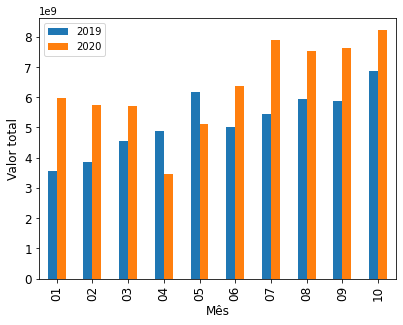
\includegraphics[scale=0.45]{images/base-de-dados-13.1-comparacao-valor-total-por-regiao.png}
        \caption{Região 1}
        \label{fig:pandemia:base-de-dados-13.1-comparacao-valor-total-por-regiao}
    \end{subfigure} ~ \quad
    \begin{subfigure}[b]{0.45\textwidth}
        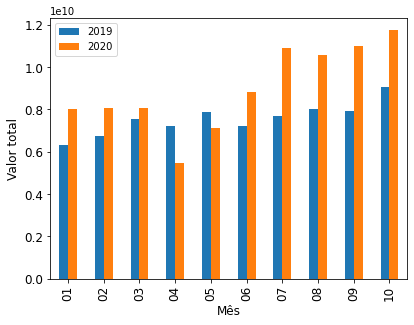
\includegraphics[scale=0.45]{images/base-de-dados-13.2-comparacao-valor-total-por-regiao.png}
        \caption{Região 2}
        \label{fig:pandemia:base-de-dados-13.2-comparacao-valor-total-por-regiao}
    \end{subfigure} ~ \\
    \begin{subfigure}[b]{0.45\textwidth}
        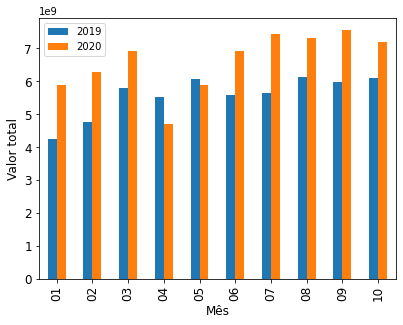
\includegraphics[scale=0.45]{images/base-de-dados-13.3-comparacao-valor-total-por-regiao.png}
        \caption{Região 3}
        \label{fig:pandemia:base-de-dados-13.3-comparacao-valor-total-por-regiao}
    \end{subfigure} ~ \quad
    \begin{subfigure}[b]{0.45\textwidth}
        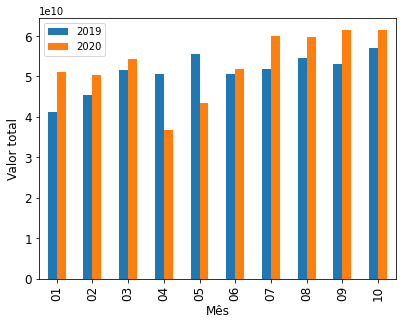
\includegraphics[scale=0.45]{images/base-de-dados-13.4-comparacao-valor-total-por-regiao.png}
        \caption{Região 4}
        \label{fig:pandemia:base-de-dados-13.4-comparacao-valor-total-por-regiao}
    \end{subfigure} ~ \\
    \begin{subfigure}[b]{0.45\textwidth} 
        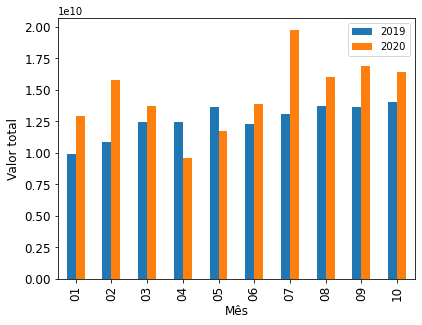
\includegraphics[scale=0.45]{images/base-de-dados-13.5-comparacao-valor-total-por-regiao.png}
        \caption{Região 5}
        \label{fig:pandemia:base-de-dados-13.5-comparacao-valor-total-por-regiao}
    \end{subfigure}
    \fdadospesquisa
\end{figure}

\begin{figure}[htb]
	\centering
    \caption{Valor total transacionado por UF no período analisado}
    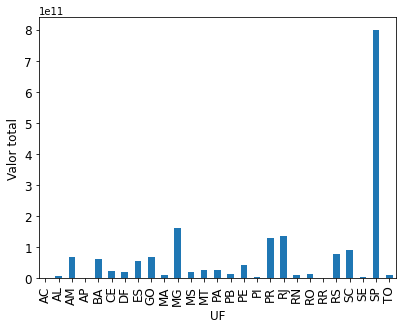
\includegraphics[scale=0.7]{images/base-de-dados-14.1-valor-total-por-uf.png}
    \label{fig:pandemia:base-de-dados-14.1-valor-total-por-uf}
    \fdadospesquisa
\end{figure}

\begin{figure}[htb]
	\centering
    \caption{Valor trimestral transacionado por UF no período analisado}
    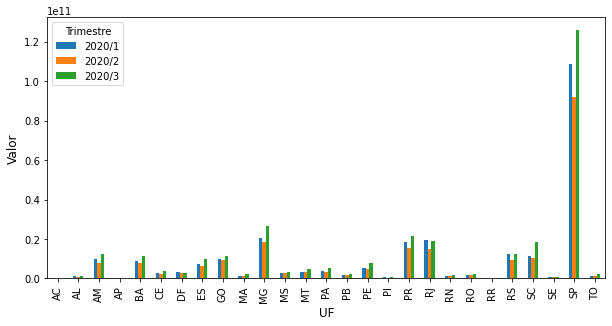
\includegraphics[scale=0.7]{images/base-de-dados-21.2-valor-trimestral-por-uf.png}
    \label{fig:pandemia:base-de-dados-21.2-valor-trimestral-por-uf}
    \fdadospesquisa
\end{figure}

\begin{table}[htb]
\centering
\caption{Diferença entre valores mensais transacionados previstos e obtidos por UF no período da pandemia}
\label{tab:pandemia:variacao-mensal-por-uf}
    \begin{tabular}{c|r|r|r|r|r|r|r|r}
        \toprule
        \textbf{UF} & Março & Abril & Maio & Junho & Julho & Agosto & Setembro & Outubro \\
        \midrule
        \textbf{AC} &  -7.3\% & -33.9\% &  -5.1\% &   9.2\% &   27.3\% &    20.5\% &    20.6\% &   15.4\% \\
        \textbf{AL} & -11.0\% & -33.6\% & -26.5\% & -12.3\% &    6.9\% &     3.9\% &    15.4\% &    9.0\% \\
        \textbf{AM} & -15.8\% & -62.5\% & -31.5\% & -14.3\% &    0.5\% &    -4.5\% &    -8.4\% &    4.1\% \\
        \textbf{AP} & -15.6\% & -29.1\% & -17.5\% &  -8.1\% &   17.4\% &    23.9\% &    22.1\% &   12.9\% \\
        \textbf{BA} &  -0.4\% & -36.0\% & -21.7\% &  -3.3\% &   11.0\% &     4.9\% &    12.7\% &   13.5\% \\
        \textbf{CE} & -15.6\% & -45.1\% & -26.3\% &  -7.7\% &   10.8\% &     7.6\% &     7.4\% &   19.1\% \\
        \textbf{DF} &  32.3\% & -18.6\% & -19.0\% &  16.4\% &    9.8\% &     2.8\% &    10.7\% &    6.6\% \\
        \textbf{ES} &  -6.5\% & -40.1\% & -24.2\% &  -5.8\% &    6.1\% &     5.6\% &    16.2\% &    6.4\% \\
        \textbf{GO} &  10.8\% & -29.5\% &  -7.9\% &   4.0\% &    9.5\% &     1.3\% &     7.3\% &    0.4\% \\
        \textbf{MA} & -20.9\% & -31.2\% & -24.8\% &   0.2\% &   22.3\% &    21.2\% &     6.8\% &   13.7\% \\
        \textbf{MG} &  -9.0\% & -35.1\% & -20.6\% &  -6.7\% &   12.2\% &     9.1\% &    12.0\% &   11.1\% \\
        \textbf{MS} &   3.4\% & -16.0\% &  -9.1\% &  -1.6\% &   12.8\% &     5.8\% &    -3.5\% &  -15.3\% \\
        \textbf{MT} & -13.3\% & -38.9\% & -13.4\% &  -3.2\% &    7.0\% &    24.5\% &    19.8\% &   17.0\% \\
        \textbf{PA} & -13.6\% & -33.3\% & -25.8\% &  -8.8\% &   18.5\% &     5.9\% &     9.7\% &    6.1\% \\
        \textbf{PB} &  -8.7\% & -38.5\% & -11.6\% &   1.7\% &   36.1\% &    15.8\% &    20.2\% &   30.7\% \\
        \textbf{PE} & -14.6\% & -43.4\% & -21.0\% &  -7.9\% &   17.5\% &    15.8\% &    11.8\% &   23.9\% \\
        \textbf{PI} & -10.6\% & -47.1\% & -24.5\% &  -7.0\% &   25.2\% &    13.4\% &    24.3\% &   15.1\% \\
        \textbf{PR} &  -2.2\% & -37.2\% & -22.8\% & -11.5\% &    1.5\% &    -0.7\% &     1.4\% &   -2.0\% \\
        \textbf{RJ} &  -6.7\% & -43.6\% & -25.6\% & -17.2\% &   -8.6\% &   -10.4\% &   -17.7\% &  -17.7\% \\
        \textbf{RN} & -14.9\% & -47.3\% & -39.7\% & -23.3\% &   10.6\% &     8.1\% &    24.7\% &   31.9\% \\
        \textbf{RO} &  -3.0\% & -25.2\% & -10.0\% &  -4.7\% &   17.1\% &     2.1\% &    -0.1\% &   -4.8\% \\
        \textbf{RR} &  82.5\% &  90.6\% & 189.3\% & 370.4\% & 1480.1\% & - & - & - \\
        \textbf{RS} & -18.4\% & -42.0\% & -33.7\% & -20.1\% &   -7.9\% &   -17.9\% &   -15.0\% &  -23.9\% \\
        \textbf{SC} &  -8.2\% & -32.5\% & -18.8\% &  -6.3\% &   89.5\% &    12.3\% &    20.3\% &   19.7\% \\
        \textbf{SE} &  -4.2\% & -38.7\% &   6.2\% &  23.9\% &   16.0\% &    13.6\% &     7.4\% &   26.6\% \\
        \textbf{SP} &  -0.9\% & -32.9\% & -24.1\% &  -9.9\% &    3.0\% &     1.9\% &     4.6\% &    4.1\% \\
        \textbf{TO} & -13.4\% & -32.1\% & -18.9\% &   2.4\% &   18.4\% &    13.9\% &    23.7\% &   19.7\% \\
        \bottomrule
    \end{tabular}
\nota{Os dados de Roraima foram insuficientes para uma previsão correta e registraram valores com bastante ruído, fazendo com que a previsão de valores utilizando a regressão linear indicasse valores bastante pessimistas para os meses da pandemia. Foram mantidos os valores de março a julho e removidos os valores posteriores devido ao ruído. Da mesma forma, consideramos que o estado de Roraima não foi impactado negativamente pela pandemia}
\fdadospesquisa
\end{table}

\begin{table}[htb]
\centering
\caption{Diferença entre valores totais transacionados previstos e obtidos por UF no período da pandemia}
\label{tab:pandemia:variacao-total-por-uf}
    \begin{tabular}{l|r}
        \toprule
        \textbf{UF} & Variação total \\
        \midrule
        \textbf{AC} &   6.2\% \\
        \textbf{AL} &  -5.5\% \\
        \textbf{AM} & -15.7\% \\
        \textbf{AP} &   1.3\% \\
        \textbf{BA} &  -1.8\% \\
        \textbf{CE} &  -5.7\% \\
        \textbf{DF} &   5.1\% \\
        \textbf{ES} &  -4.9\% \\
        \textbf{GO} &  -0.4\% \\
        \textbf{MA} &  -0.7\% \\
        \textbf{MG} &  -3.1\% \\
        \textbf{MS} &  -2.9\% \\
        \textbf{MT} &   0.4\% \\
        \textbf{PA} &  -4.6\% \\
        \textbf{PB} &   5.9\% \\
        \textbf{PE} &  -1.7\% \\
        \textbf{PI} &  -0.7\% \\
        \textbf{PR} &  -8.9\% \\
        \textbf{RJ} & -18.4\% \\
        \textbf{RN} &  -6.1\% \\
        \textbf{RO} &  -3.4\% \\
        \textbf{RR} & 484.7\% \\
        \textbf{RS} & -22.1\% \\
        \textbf{SC} &  10.0\% \\
        \textbf{SE} &   6.6\% \\
        \textbf{SP} &  -6.6\% \\
        \textbf{TO} &   2.5\% \\
        \bottomrule
    \end{tabular}
\fdadospesquisa
\end{table}

\begin{table}[htb]
\centering
\caption{Quantidade de UFs impactadas negativamente pela pandemia em relação às variações mensais ou totais}
\label{tab:pandemia:impacto-por-uf}
    \begin{tabular}{l|r|r}
        \toprule
        Impacto & Mensal & Total \\
        \midrule
        Sim & 24 & 18 \\
        Não &  3 &  9 \\
        \bottomrule
    \end{tabular}
\fdadospesquisa
\end{table}

\section{Cenário setorial}

\begin{figure}[htb]
	\centering
    \caption{Valor total transacionado por seção no período analisado}
    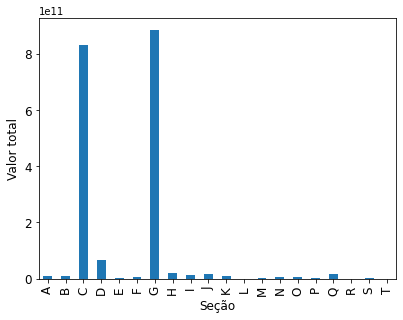
\includegraphics[scale=0.7]{images/base-de-dados-15.1-valor-total-por-secao.png}
    \label{fig:pandemia:base-de-dados-15.1-valor-total-por-secao}
    \fdadospesquisa
\end{figure}

\begin{figure}[htb]
	\centering
    \caption{Valor trimestral transacionado por seção no período analisado}
    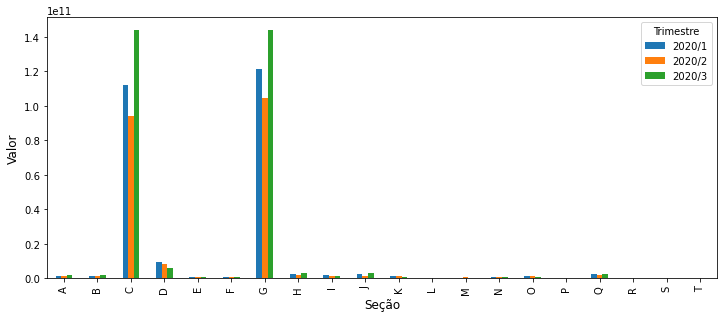
\includegraphics[scale=0.7]{images/base-de-dados-22-valor-trimestral-por-secao.png}
    \label{fig:pandemia:base-de-dados-22-valor-trimestral-por-secao}
    \fdadospesquisa
\end{figure}

\begin{table}[htb]
\centering
\caption{Diferença entre valores mensais transacionados previstos e obtidos por seção no período da pandemia}
\label{tab:pandemia:variacao-mensal-por-secao}
    \begin{tabular}{c|r|r|r|r|r|r|r|r}
        \toprule
        \textbf{Seção} & Março & Abril & Maio & Junho & Julho & Agosto & Setembro & Outubro \\
        \midrule
        \textbf{A} & -15.4\% & -24.4\% & -14.2\% & -10.8\% &   6.9\% &   8.2\% &  32.9\% &  28.6\% \\
        \textbf{B} &   2.8\% &  12.8\% &  19.1\% &  32.7\% &  50.6\% &  51.0\% &  58.5\% &  64.6\% \\
        \textbf{C} &  -4.2\% & -39.0\% & -23.6\% &  -5.8\% &  16.0\% &  11.7\% &  15.5\% &  16.2\% \\
        \textbf{D} &  -1.4\% &  -6.1\% & -16.7\% & -14.4\% & -12.8\% & -39.3\% & -62.2\% & -64.5\% \\
        \textbf{E} &  10.8\% & -32.0\% & -17.3\% &  17.1\% &  65.5\% & 125.2\% &  -1.3\% &  15.3\% \\
        \textbf{F} &  -4.7\% & -30.0\% & -26.8\% & -20.0\% &  -8.1\% & -13.8\% & -10.0\% & -15.0\% \\
        \textbf{G} &  -5.9\% & -36.8\% & -23.0\% & -11.6\% &   4.0\% &  -2.3\% &  -0.2\% &  -2.3\% \\
        \textbf{H} & -16.2\% & -40.0\% & -39.2\% & -24.5\% & -17.0\% & -15.5\% &  -7.0\% &  -9.7\% \\
        \textbf{I} & -25.8\% & -53.7\% & -51.7\% & -42.2\% & -33.1\% & -33.4\% & -27.9\% & -25.3\% \\
        \textbf{J} &  24.3\% & -61.6\% & -47.4\% & -32.3\% &  -6.4\% &  -5.3\% & -19.3\% &   5.4\% \\
        \textbf{K} &   4.6\% &  15.1\% &  12.6\% &  13.2\% &  14.2\% & -72.6\% & -64.8\% & -66.1\% \\
        \textbf{L} & -28.3\% & -34.7\% & -56.8\% & -51.3\% & -49.2\% & -29.1\% & -34.2\% & -57.0\% \\
        \textbf{M} & -12.2\% & -12.2\% &  57.9\% &  71.4\% & -33.2\% & -32.2\% & -16.3\% & -12.8\% \\
        \textbf{N} &  -1.6\% & -52.1\% & -42.2\% & -10.0\% &  28.9\% &  -4.7\% &   5.7\% &   1.9\% \\
        \textbf{O} &  53.8\% &  20.7\% &   2.8\% &  77.7\% &  11.1\% &  -4.6\% &  27.2\% & -28.1\% \\
        \textbf{P} & -12.0\% & -56.8\% & -44.6\% & -33.5\% & -22.1\% & -34.0\% & -31.3\% & -39.5\% \\
        \textbf{Q} &  33.1\% & -10.5\% &  -6.4\% &  -7.2\% &   6.7\% &  -3.9\% &   2.7\% & -11.2\% \\
        \textbf{R} & -32.2\% & -68.9\% & -69.6\% & -50.6\% & -42.7\% & -41.5\% & -18.5\% & -18.3\% \\
        \textbf{S} &  -5.4\% & -32.9\% & -24.7\% & -22.5\% & -10.4\% & -19.5\% &   2.0\% &  -0.2\% \\
        \textbf{T} & -40.5\% & -38.2\% & -61.9\% & -48.5\% & -47.5\% & -54.7\% & -54.2\% & -27.6\% \\
        \bottomrule
    \end{tabular}
\fdadospesquisa
\end{table}

\begin{table}[htb]
\centering
\caption{Diferença entre valores totais transacionados previstos e obtidos por seção no período da pandemia}
\label{tab:pandemia:variacao-total-por-secao}
    \begin{tabular}{l|r}
        \toprule
        \textbf{Seção} & Variação total \\
        \midrule
        \textbf{A} &   2.4\% \\
        \textbf{B} &  36.0\% \\
        \textbf{C} &  -1.3\% \\
        \textbf{D} & -27.0\% \\
        \textbf{E} &  23.5\% \\
        \textbf{F} & -16.0\% \\
        \textbf{G} &  -9.5\% \\
        \textbf{H} & -20.8\% \\
        \textbf{I} & -36.5\% \\
        \textbf{J} & -17.4\% \\
        \textbf{K} & -17.7\% \\
        \textbf{L} & -42.8\% \\
        \textbf{M} &   0.5\% \\
        \textbf{N} &  -9.1\% \\
        \textbf{O} &  20.8\% \\
        \textbf{P} & -34.2\% \\
        \textbf{Q} &   0.3\% \\
        \textbf{R} & -42.7\% \\
        \textbf{S} & -14.0\% \\
        \textbf{T} & -46.6\% \\
        \bottomrule
    \end{tabular}
\fdadospesquisa
\end{table}

\begin{table}[htb]
\centering
\caption{Quantidade de seções impactadas negativamente pela pandemia em relação às variações mensais ou totais}
\label{tab:pandemia:impacto-por-secao}
    \begin{tabular}{l|r|r}
        \toprule
        Impacto & Mensal & Total \\
        \midrule
        Sim & 17 & 14 \\
        Não &  3 &  6 \\
        \bottomrule
    \end{tabular}
\fdadospesquisa
\end{table}

\begin{figure}[htb]
	\centering
    \caption{Histograma do valor total transacionado por CNAE no período analisado}
    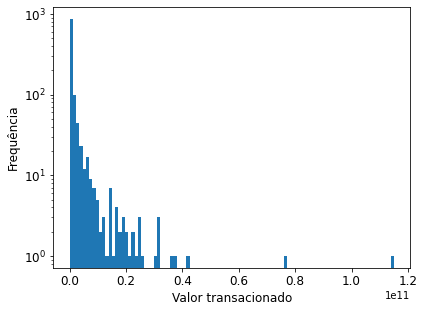
\includegraphics[scale=0.7]{images/base-de-dados-23.1-valor-total-por-cnae.png}
    \label{fig:pandemia:base-de-dados-23.1-valor-total-por-cnae}
    \fdadospesquisa
\end{figure}

\begin{figure}[htb]
	\centering
    \caption{Diagrama de caixa dos valores mensais transacionados por CNAE no período analisado}
    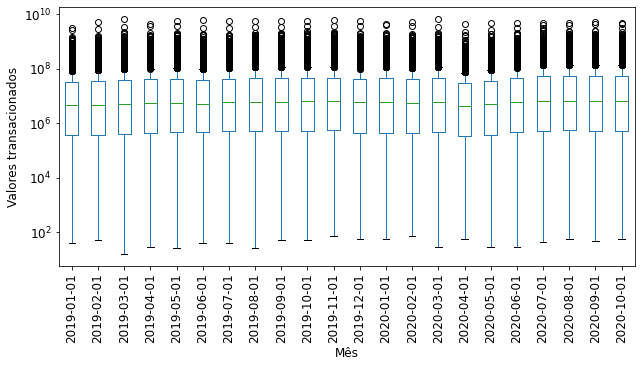
\includegraphics[scale=0.7]{images/base-de-dados-23.2-valor-mensal-por-cnae.png}
    \label{fig:pandemia:base-de-dados-23.2-valor-mensal-por-cnae}
    \fdadospesquisa
\end{figure}

\begin{table}[htb]
\centering
\caption{Quantidade de CNAEs impactadas negativamente pela pandemia em relação às variações mensais ou totais}
\label{tab:pandemia:impacto-por-cnae}
    \begin{tabular}{l|r|r}
        \toprule
        Impacto & Mensal & Total \\
        \midrule
        Sim & 852 & 600 \\
        Não & 273 & 525 \\
        \bottomrule
    \end{tabular}
\fdadospesquisa
\end{table}
